\chapter{Introduction}\label{chapter_introduction}
\lettrine{R}{eal-time embedded} systems are usually characterized by timely computation, which is identified as  \textit{Deadline}, besides correct output of the computation~\cite{butazzo}. They are applied in many safety-critical applications, e.g., the braking system in vehicles, besides applying the appropriate force on the wheel, the time taken to slow down (or halt) the vehicle must be timely otherwise accident can occur. Therefore, safety-critical real-time systems should be analyzed rigoruously for functional safety, for instance, the ISO 26262 standard ``Road vehicles-Functional safety''~\cite{iso201126262} suggests early analysis of automotive systems, that is during requirements specification and software design, and the use of formal methods, which are mathematical techniques and tools that enable unambiguous specification and modeling, and rigorous analysis of systems~\cite{o2017concise}.

In distributed computing, the safety-critical software is mapped on multiple hardware systems to capitalize on the computational power provided by the distributed architecture, e.g., the executing of the braking software on multiple electronic control units (ECU). Since the distributed software is  normally exposed to a greater degree of permanent and transient faults, reliability of the safety-critical software should be maximized to improve dependability of the  system which requires additional critical systems resource such as power and energy besides computational resources. However, the embedded hardware is usually resource constrained, therefore, the software should be efficiently mapped to the hardware to conserve critical system resources, but also to accommodate current and future growth of the software functionality.

In this thesis, we apply formal methods to improve the requirements specifications of safety-critical systems, and to analyze the functional and timing of the safety-critical software against the specifications. Safety-critical requirements specifications should be unambiguous, comprehensible, etc. In fact, according standards, e.g., ISO 26262, semi-formal or formal languages are recommended to specify safety-critical requirements. However, natural language is the de facto method to specify embedded systems requirements industry because it is intuitive and expressive. However, it is inherently ambiguous, consequently the natural language specifications are sometimes ambiguous, incomprehensible, inconsistent, etc~\cite{ieereqspecstandard}. Template-based specification and controlled natural language are the two most commonly used methods to improve requirements specifications. The template-based specification methods, e.g., requirements boilerplates~\cite{Hull2011RequirementsEngineering}, etc.,  lack meta-model for extensible and the template selection is usually cumbersome. Controlled natural languages, e.g., Attempto~\cite{attempto96}\cite{Fuchs2008AttemptoRepresentation}, etc., mimic the intuitiveness of natural language and have formal semantics, however, lacks support for embedded systems, hence are less effective. In this thesis, we propose a constrained natural language which is domain-specific and uses the notion of boilerplates to facilitate reuse. The specifications have semantics in Boolean logic and description logic to enable rigoruous analysis via Boolean satisfiability and ontology, respectively.

The specifications are employed in subsequent system development including software design to verify the latter for correct functionality. The software design is usually modeled, simulated and analyzed before implementation. In this regard, Simulink is one of the most widely used development environment for multi-domain, multi-rate, discrete and continuous safety-critical systems in industry~\cite{JamesB.Dabney2003MasteringSimulink}. For this main reason, there is increasing interest in formal analysis of Simulink models~\cite{Manamcheri2011AModels}\cite{Sims2007ExperienceReport}. Simulink Design Verifier, which is based on the Prover model-checker, is the de facto tool in the Simulink environment to formally verify Simulink design models. However, it has limited functionality, e.g., it supports only discrete models, has issues with scalability, and lacks verification of timed properties.  We propose transformation of Simulink models to network of stochastic time, subsequently analyzing the latter via statistical model checking, which is uses traces of executions and statistical analysis technques, e.g., monte-carlo simulation, etc., to check properties, that is in contrast to exhaustive model checking. The statistical model checking is shown to scale well on complex and large problems unlike the exact model checking, which suffers from state-space explosion.

The software design is mapped to hardware, which should take into consideration effectiveness and efficiency. The software should be effectively mapped to the execution platform, that is satisfying the timing and reliability requirements of a distributed safety-critical software. The timing considers fixed-priority preemptive scheduling of tasks, the end-to-end delay of chains (or sequence of tasks), and the reliability maximization employs fault tolerance via active replication of software components on different computing units. Furthermore, the allocation should be efficient so that the power consumption is minimized to ensure extensibility of the software, that is to accommodate future growth of the software functionality, which is evident for instance in the automotive electical/electronic systems where hundreds of software functions are executed. The software-to-hardware allocation problem is NP-hard, so the exact methods, which deliver optimal solutions, e.g., branch and bound, dynamic programming, etc., are usually used for relatively small problems. On the other hand, heuristics, which deliver near-optimal solutions, are applied on large and complex problems. We propose formulation of the software allocation as an integer-linear programming, subsequently solve via branch and bound Furthermore, we propose hybrid-particle optimization to solve large software allocation problems.

\section{Research Contributions Overview}
In this subsection, we give overview of the thesis contributions, and later in Section x, the contributions are further discussed in detail.
\begin{itemize}
\item \textbf{Formal Analysis of natural language requirements:}  we propose a fairly expressive, flexible yet structured and domain-specific constrained natural language, called \textit{ReSA}~\cite{resatool}\cite{Mahmud2015ReSA:Systems}. The language has semantics in Boolean and description logic to support for shallow and rigorous analysis, respectively. The Boolean specifications are checked for consistency using the satisfiability-modulo theory via the Z3 SMT solver. Whereas, the description logic is used to encode the specification as ontology, where we check consistency of the specifications at the lexical level using Reasoner (Inference engine) such Hermit. The ReSA tool, which consists of an editor and implements consistency-checking functionality, is integrated seamlessly into EATOP, which is an open source EAST-ADL IDE, to complement the requirements modeling. 

\item \textbf{Scalable analysis of Simulink models:} we propose a pattern-based, execution-order preserving automatic transformation of atomic and composite Simulink blocks into stochastic timed automata that can be formally analyzed using UPPAAL Statistical Model Checker \cite{Bulychev2012UPPAAL-SMC:Automata}. Our method is scalable, and has been validated on industrial use cases \cite{Filipovikj2016SimulinkSystems}. The statistical model checker analyzes a state-transition system by conducting statistical analysis on the collected traces of the system executions, effectively mitigating the state-space explosion of (exact) model checking \cite{Legay2010StatisticalOverview}. 

\item \textbf{Efficient Power consumption ILP and metaheuristics:} we propose an integer-linear programming (ILP) model to the allocation of distributed software on the network of heterogeneous computing units, which have different processor speed, failure rate and power consumption specifications. The ILP implemented in JAVA using the ILOG CPLEX interface, and subsequently solved the CPLEX solver.
\item \textbf{Validation on industrial use cases: } 
Our contributions such as its the ReSA language as well as the proposed formal analysis of Simulink model is validated on industrial use cases, which are provided
%\end{itemize}
% \begin{figure}
% 	\centering
% 	\ifpdf
% 	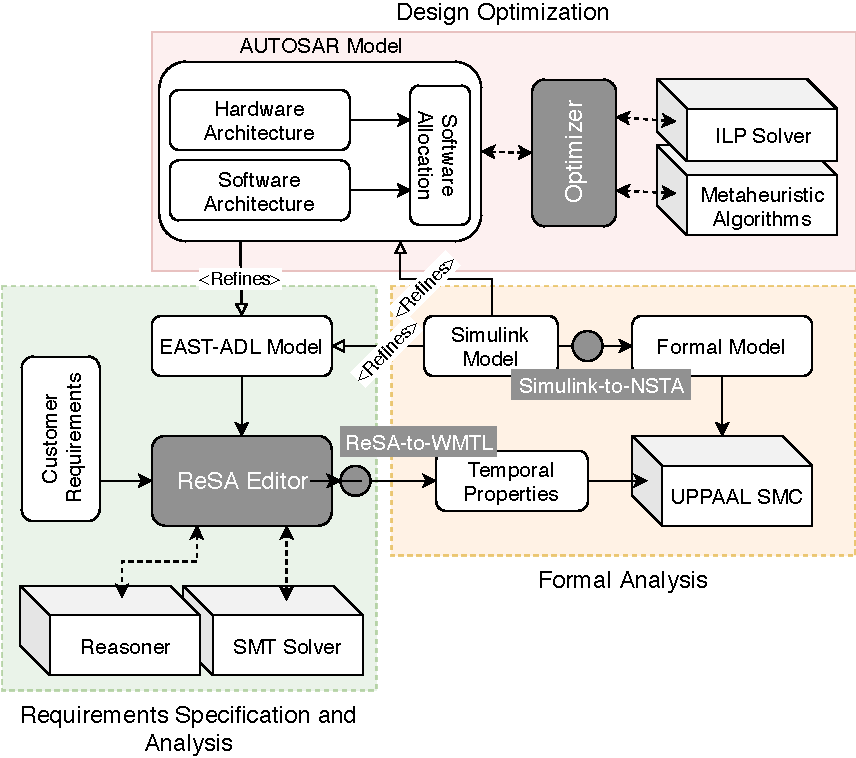
\includegraphics[width=\linewidth]{images/softdevflow}
% 	\else
% 	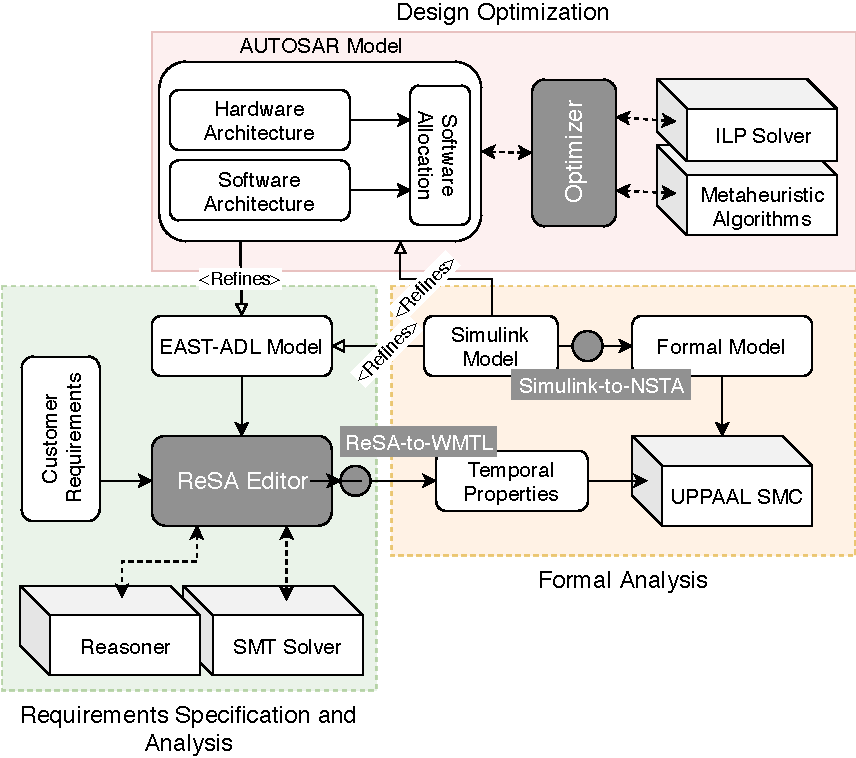
\includegraphics[width=1.0\linewidth]{images/softdevflow.eps}
% 	\fi
% 	\caption{Thesis Contributions Workflow.} 
% \end{figure}

Our solutions are evaluated on industrial automotive use cases and on a realistic benchmark. The formal analysis of the natural language requirements specifications in ReSA and the formal analysis of Simulink models are evaluated on the adjustable speed-limiter (ASL) and brake-by-wire (BBW) systems provided by Volvo Group Trucks Technology (VGTT). ASL is a speed-limitation automotive function which controls the vehicle speed of Volvo trucks from speeding up, and is useful in roads where speed-limitation signs are in place. The ASL use case consists of around 300 requirements, which are specified in natural language, architectural models in EAST-ADL and Simulink models. The integrated software allocation is evaluated on the engine management system benchmark provided by Bosch~\cite{} provided for AUTOSAR applications. The benchmark consists of statistics of the schedulable objects, such as mean values, shars of timing specifications and activation mechanisms of the schedulable objects in the system.

\section{Thesis Outline Overview}
The thesis is divided into two parts. The first part is a summary of our research. It is organized as follows: in Chapter 2, we give the background information on description logic, Boolean satisfiability problem, Simulink, stochastic timed automata, and meta-heuristic optimization. In Chapter 3, we explain the research problem and outline the research goals. The thesis contributions are discussed in Chapter 4, followed by the related work in Chapter 5. In Chapter 3, we describe the research method applied to conduct the research. Finally, in Chapter 7, we conclude the thesis and outline possible directions for future work.
